\documentclass[12pt]{article}
\usepackage[ngerman]{babel}
\usepackage{amsmath}
\usepackage[utf8]{inputenc}
\usepackage{hyperref}
\usepackage{setspace}
\setstretch{1.5}
\usepackage[paper=a4paper,left=25mm,right=35mm,top=25mm,bottom=20mm]{geometry}
\usepackage{graphicx}

\hypersetup{
    colorlinks,
    citecolor=black,
    filecolor=black,
    linkcolor=black,
    urlcolor=black
}

\begin{document}

\title{Extremwertproblem Wegfindung \\  \large{\enspace Vergleich verschiedener Algorithmen}}

\author{Maximilian Stark}

\maketitle
\thispagestyle{empty}
\clearpage

\tableofcontents
\thispagestyle{empty}
\clearpage

\section{Einleitung}
\newpage

\section{Grundlagen und Terminologie}
Zu Beginn werden in diesem Abschnitt die grundlegenden Begriffe der Graphen-Theorie geklärt. Auch Fachbegriffe aus der Implementierung durch die Informatik werden erläutert.
\\
Das Ziel dieser Arbeit ist die Darstellung und der Vergleich verschiedener \textit{Wegfindungs-Algorithmen} in der Anwendung an verschiedenen generierten\textit{Graphen}.
\\\\
Zugrunde all dem liegt die Graphen-Theorie. Deren Fundament ist der namensgebende \textit{Graph} $G\; = \{V,\,E\}$, welcher aus einer Menge von \textit{Knoten} $V$ (von engl. "`Vertex") und aus einer Menge \textit{Kanten} $E$ (von engl. "`Edge").
\\
Zeichnerisch werden \textit{Knoten} als Punkte oder Kreise dargestellt; \textit{Kanten} als Verbindungslinien zwischen zwei \textit{Knoten}. Jede \textit{Kante} hat einen \textit{Startknoten} und einen \textit{Endknoten}. Wenn von einer \textit{gerichteten Kante} die Rede ist, lässt sich das als Pfeil interpretieren, da die Verbindung unidirektional gilt. Ebenso gibt es die \textit{gewichteten Kanten}, denen nicht nur zwei \textit{Knoten} zugeordnet werden, sondern zusätzlich noch ein Gewicht $w$ (von engl. "`Weight"), ein Zahlenwert, der als Kosten der Beziehung zwischen den beiden \textit{Knoten} gesehen werden kann.
\\
In der Wegfindung ist ein \textit{Weg} $P$ (von engl. "`Path") als geordnete Abfolge von \textit{Knoten} definiert. Da in der Regel jedes \textit{Knoten}-Paar nur einfach verbunden ist, reicht in der Implementierung dieser Ansatz aus.
\\
Visuell wird der \textit{Graph} durch einen \textit{Layout-Algorithmus} dargestellt, welcher allen \textit{Knoten} durch gewisse Berechnungen Positionen zuteilt. Mehr dazu in Abschnitt \ref{sec:layout}.
\\
Generell sind \textit{Algorithmen} eine festgelegte Abfolge von Schritten um Daten zu verarbeiten. In der Informatik sind diese einzelnen Schritte Befehle.
\newpage
\section{Aufbau und Bedienung des Programms}
Das Programm, im eigentlichen Fokus stehend, fungiert sowohl als visuelle Möglichkeit der Darstellung, als auch als Quelle für Vergleichsdaten und Messungen in selbst erzeugten Szenarien.
Geschrieben ist das Programm in der Programmiersprache \textit{Java} unter Verwendung der \textit{JavaFX}-Standardbibliothek \cite{javafx}.
\begin{figure}[h!]
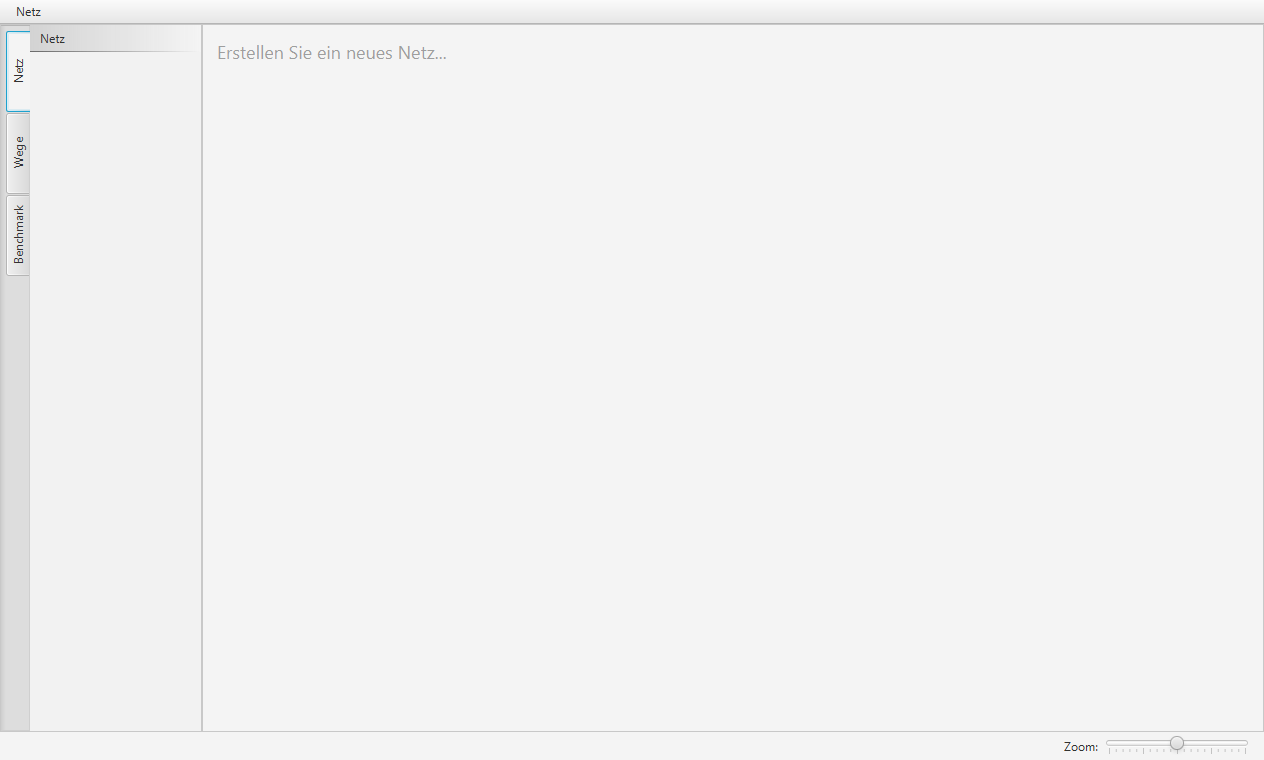
\includegraphics[width=\textwidth]{res/main_screenshot.png}
\centering
\caption{Die Start- und Hauptansicht der Applikation}
\label{fig:main_screenshot}
\end{figure}
\\
Auf den ersten Blick ist die Anwendungsoberfläche in zwei größere Bereiche aufgeteilt. Im linken, kleineren Seitenbereich werden detaillierte Informationen über den \textit{Graphen}, bereits berechnete \textit{Wege} und die Konfigurationsmöglichkeiten neuer Wege, in mehreren "`Tabs" unterteilt, angezeigt. Der große rechte Bereich, zu Beginn der Anwendung nur mit "`Erstellen Sie ein neues Netz..." (siehe Abb.~\ref{fig:main_screenshot}) beschriftet, dient als Hauptansicht von sowohl des Graphen, als auch der Vergleichsstatistiken und Tabellen.
\\
Die Bedienung kann vollständig mit der Maus erfolgen, da sich sämtliche Features visuell intuitiv und minimalistisch präsentieren. Nur vereinzelt führen Tastatureingaben oder "`Hotkeys" zu mehr Komfort oder Genauigkeit der Anwendung. 
\newpage
-
\newpage
\section{Konstruktion des Graphen}
Im nächsten Schritt werden wir nun einen Graphen erzeugen lassen und die Funktionsweise des Generators betrachten.
\newpage

\section{Visuelles Layout des Graphen}
\label{sec:layout}
\newpage

\section{Wegfindungs-Algorithmen}
\newpage

\subsection{Gröbste Züge von Intelligenz: Tiefensuche}
\newpage
-
\newpage

\subsection{Heuristik als Mittel zum Ziel: Der Dijkstra-Algorithmus}
\newpage
-
\newpage

\subsection{Der Allstar: Der A*-Algorithmus}
\newpage
-
\newpage

\section{Vergleichsstatistik und Fazit}
\newpage
-
\newpage

\section{Schluss}
\newpage

\begin{thebibliography}{9}
\bibitem{javafx} JavaFX-Homepage http://docs.oracle.com/javase/8/javafx/get-started-tutorial/jfx-overview.htm \emph{abgerufen am 14.10.15}
\end{thebibliography}

\end{document}
